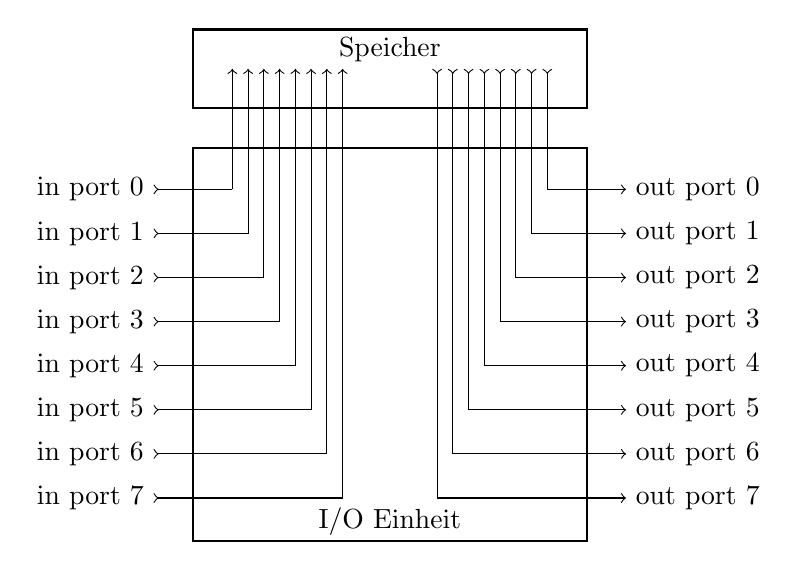
\begin{tikzpicture}  
  \draw[thick] (0,0) rectangle (5,5);
  \node at     (2.5,0.25) {I/O Einheit};
  
  \foreach \y [count=\i from 0, evaluate=\i as \p using int(7-\i),
                                evaluate=\i as \s using (0.5 + \p/5),
                                evaluate=\i as \q using (4.5 - \p/5)]
  in {0.55, 1.11, ...,5}
  {
      \draw[->] (4.5, \y) -- ++(+1,0) node [right] {out port \p};
      \draw[-<] (0.5, \y) -- ++(-1,0) node [left]  {in port  \p};
      \draw[->] (0.5, \y) -| (\s,6);
      \draw[>-] (\q,6)    |- (4.5,\y);
  }
  
  \draw[thick] (0,5.5) rectangle (5,6.5);
  \node at     (2.5, 6.25) {Speicher};

\end{tikzpicture}
 
